\documentclass[
	% -- opções da classe memoir --
	12pt,				% tamanho da fonte
	openright,			% capítulos começam em pág ímpar (insere página vazia caso preciso)
	oneside,			% para impressão em recto e verso. Oposto a twoside
	a4paper,			% tamanho do papel. 
	% -- opções da classe abntex2 --
	%chapter=TITLE,		% títulos de capítulos convertidos em letras maiúsculas
	%section=TITLE,		% títulos de seções convertidos em letras maiúsculas
	%subsection=TITLE,	% títulos de subseções convertidos em letras maiúsculas
	%subsubsection=TITLE,% títulos de subsubseções convertidos em letras maiúsculas
	% -- opções do pacote babel --
	english,			% idioma adicional para hifenização
	french,				% idioma adicional para hifenização
	spanish,			% idioma adicional para hifenização
	brazil				% o último idioma é o principal do documento
	]{abntex2UFMT}

\usepackage{lmodern}			% Usa a fonte Latin Modern			
\usepackage[T1]{fontenc}		% Selecao de codigos de fonte.
\usepackage[utf8]{inputenc}		% Codificacao do documento (conversão automática dos acentos)
\usepackage{indentfirst}		% Indenta o primeiro parágrafo de cada seção.
\usepackage{color}				% Controle das cores
\usepackage{graphicx}			% Inclusão de gráficos
\usepackage{microtype} 			% para melhorias de justificação
\usepackage[a4paper]{geometry}  % definir margem
\usepackage{lipsum}				% para geração de dummy text
\usepackage[brazilian,hyperpageref]{backref}	 % Paginas com as citações na bibl
\usepackage[alf,abnt-emphasize = bf]{abntex2cite}	% Citações padrão ABNT %colocar 'num' no lugar de 'alf' para ter referencias numericas
\usepackage{fancyhdr,amsmath,amssymb,amsthm,dcolumn,wrapfig,blindtext}
\usepackage{calc,siunitx,booktabs,pifont,bigstrut,multirow,array}
\usepackage{tabularx,svg,graphicx,epstopdf,ragged2e}
\usepackage{url16023} %pacore url sem <>


\geometry{verbose,tmargin=3cm,bmargin=2cm,lmargin=3cm,rmargin=2cm} % margem
\renewcommand{\backrefpagesname}{Citado na(s) página(s):~}
\renewcommand{\backref}{}
\renewcommand*{\backrefalt}[4]{
	\ifcase #1 %
		Nenhuma citação no texto.%
	\or
		Citado na página #2.%
	\else
		Citado #1 vezes nas páginas #2.%
	\fi}%


% ---
% Informações de dados para CAPA e FOLHA DE ROSTO
% ---
\titulo{TÍTULO DO TRABALHO:\\ SUBTÍTULO DO TRABALHO \textcolor{red}{(se houver)}}

\autor{NOME E SOBRENOME}

\local{CUIABÁ - MT}

\data{202X}

\orientador{Prof. Dr. Nome e Sobrenome}

\coorientador{Prof.ª Dr.ª  Nome e Sobrenome \textcolor{red}{(se houver)}}

\instituicao{UNIVERSIDADE FEDERAL DE MATO GROSSO\\ INSTITUTO DE FÍSICA\\ PÓS-GRADUAÇÃO EM FÍSICA}

\tipotrabalho{Dissertação/Tese}

\preambulo{Tese/Dissertação apresentada ao curso de Pós-Graduação em Física do Instituto de Física da Universidade Federal de Mato Grosso como requisito parcial para a obtenção do título de doutor/mestre em Física. 
}
% ---


% ---
% Configurações de aparência do PDF final

% alterando o aspecto da cor azul
\definecolor{blue}{RGB}{41,5,195}

% informações do PDF
\makeatletter
\hypersetup{
     	%pagebackref=true,
		pdftitle={\@title}, 
		pdfauthor={\@author},
    	pdfsubject={\imprimirpreambulo},
	    pdfcreator={LaTeX with abnTeX2},
		pdfkeywords={abnt}{latex}{abntex}{abntex2}{trabalho acadêmico}, 
		colorlinks=true,       		% false: boxed links; true: colored links
    	linkcolor=black,          	% color of internal links
    	citecolor=black,        		% color of links to bibliography
    	filecolor=black,      		% color of file links
		urlcolor=black,
		bookmarksdepth=4
}
\makeatother
% --- 

% ---
% Posiciona figuras e tabelas no topo da página quando adicionadas sozinhas
% em um página em branco. Ver https://github.com/abntex/abntex2/issues/170
\makeatletter
\setlength{\@fptop}{5pt} % Set distance from top of page to first float
\makeatother
% ---

% --- 
% Espaçamentos entre linhas e parágrafos 
% --- 

% O tamanho do parágrafo é dado por:
\setlength{\parindent}{1.3cm}

% Controle do espaçamento entre um parágrafo e outro:
\setlength{\parskip}{0.2cm}  % tente também \onelineskip

% ----
% Início do documento
% ----
\begin{document}

% Seleciona o idioma do documento (conforme pacotes do babel)
%\selectlanguage{english}
\selectlanguage{brazil}

% Retira espaço extra obsoleto entre as frases.
\frenchspacing 

% ----------------------------------------------------------
% ELEMENTOS PRÉ-TEXTUAIS
% ----------------------------------------------------------

% ---
% Capa
% ---
\imprimircapa
% ---

% ---
% Folha de rosto
% (o * indica que haverá a ficha bibliográfica)
% ---
\imprimirfolhaderosto*
% ---

% ---
% Inserir a ficha bibliografica
% ---

% A biblioteca da sua universidade lhe fornecerá um PDF
% com a ficha catalográfica definitiva após a defesa do trabalho. Quando estiver
% com o documento, salve-o como PDF no diretório do seu projeto e substitua todo
% o conteúdo de implementação deste arquivo pelo comando abaixo:
%
% \begin{fichacatalografica}
%     \includepdf{fig_ficha_catalografica.pdf}
% \end{fichacatalografica}

\begin{fichacatalografica}

\noindent\textcolor{red}{A ficha catalográfica pode ser elaborada
no site https://academico-siga.ufmt.br/ufmt.sfc/ Home seguindo as
orientações que constam na página do sistema. Atentem-se ao uso de
letras maiúsculas e minúsculas seguindo os exemplos nos campos de
preenchimento, bem como as orientações sobre o campo de Nome (onde
deve usar toda a extensão do nome exceto o último sobrenome e grau
de parentesco), o campo de Último Sobrenome, como indicado deve conter
o último sobrenome do autor e caso haja grau de parentesco, como Júnior,
Neto, Filha entre outros dessa natureza devem estar nesse campo também.}

\noindent\textcolor{red}{O autor deve observar também se a ficha
gerada apresenta todas as informações que foram preenchidas no sistema,
caso contrário deve utilizar o recurso de \textquotedblleft tamanho
de fonte\textquotedblright{} para que todas fiquem visíveis no quadro
da ficha}

\vspace{0.15\linewidth}

\begin{center}
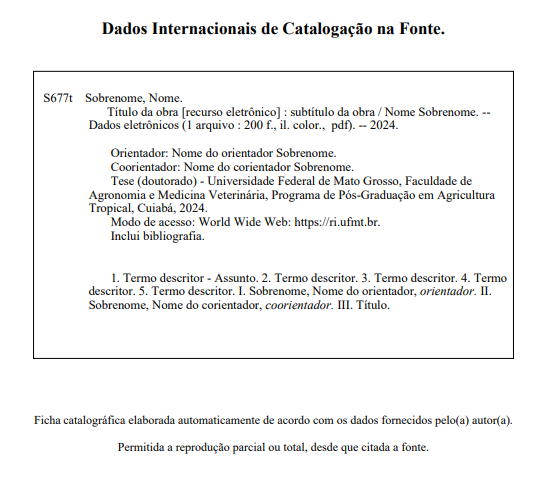
\includegraphics[scale=0.75]{figs/ficha.png}
\par\end{center}

\end{fichacatalografica}
% ---

% ---
% Inserir folha de aprovação
% ---

% Isto é um exemplo de Folha de aprovação, elemento obrigatório da NBR
% 14724/2011 (seção 4.2.1.3). Você pode utilizar este modelo até a aprovação
% do trabalho. Após isso, substitua todo o conteúdo deste arquivo por uma
% imagem da página assinada pela banca com o comando abaixo:
%
% \begin{folhadeaprovacao}
% \includepdf{folhadeaprovacao_final.pdf}
% \end{folhadeaprovacao}
%
\begin{folhadeaprovacao}

  \begin{center}
    {\large\imprimirautor}

    \vspace*{\fill}
    \begin{center}
      \large\imprimirtitulo
    \end{center}
    \vspace*{\fill}
    
    \hspace{.45\textwidth}
    \begin{minipage}{.5\textwidth}
        \imprimirpreambulo
    \end{minipage}%
    \vspace*{\fill}
   \end{center}
        
   \begin{center}
   Aprovado em XX de XX de 20XX
   \par\end{center}

   \assinatura{Presidente da Banca/Orientador: Doutor(a) Nome e Sobrenome \\ Instituição: Universidade Federal de Mato Grosso} 
   \assinatura{Examinador Interno: Doutor(a) Nome e Sobrenome \\ Instituição: Universidade Federal de Mato Grosso}
   \assinatura{Examinadora Externa: Doutor(a) Nome e Sobrenome \\ Instituição: Nome da Instituição}
   %\assinatura{Professor \\ Convidado 3}
   %\assinatura{Professor \\ Convidado 4}
      
   \begin{center}
    \noindent\textcolor{red}{Folha de aprovação é um elemento obrigatório. Recomendamos que na versão final do trabalho conste a folha de aprovação assinada, seja de forma manual (digitalizada), seja de forma eletrônica (assinaturas via Sistema SEI)}
  \end{center}
  
\end{folhadeaprovacao}
% ---

% ---
% Dedicatória
% ---
\begin{dedicatoria}

   \vspace*{\fill}
   \centering
   \noindent\textcolor{red}{(A dedicatória é um elemento opcional. Esta parte não tem título no topo, e caso seja usada deve ser evidenciada com o uso de termos que indiquem uma dedicação)}
   \vspace*{\fill}
   
    \begin{flushright}
    Dedico este trabalho a XXX
    \par\end{flushright}
    
\end{dedicatoria}
% ---

% ---
% Agradecimentos
% ---
\begin{agradecimentos}
Agradeço a XXX

   \vspace*{\fill}
   \centering
   \noindent\textcolor{red}{(Agradecimentos é um elemento opcional)}
   \vspace*{\fill}

\end{agradecimentos}
% ---

% ---
% Epígrafe
% ---
\begin{epigrafe}
    \vspace*{\fill}

	\noindent\textcolor{red}{A epígrafe é um elemento opcional e a citação deve ter alguma relação com o tema do trabalho desenvolvido, seguido de sua autoria. Deve ser elaborada de acordo com a NBR 10520.}
    \begin{flushright}
    \noindent\textcolor{red}{(Autor, ano)}
	\end{flushright}
\end{epigrafe}
% ---

% ---
% RESUMOS
% ---

% resumo em português
\setlength{\absparsep}{18pt} % ajusta o espaçamento dos parágrafos do resumo
\begin{resumo}
Este é um elemento obrigatório que deve ser elaborado conforme a ABNT NBR 6028. Nesta norma é possível identificar o tipo de resumo indicado entre outras informações para a construção do mesmo. Deve ser apresentado utilizando parágrafo único, espaçamento entre linhas simples e tamanho da fonte 12. Deve conter de 150 a 500 palavras. Abaixo do resumo deve-se informar até 5 palavras-chaves separadas por ponto e vírgula e finalizada com ponto. 

 \textbf{Palavras-chave}: palavra-chave 1; palavra-chave 2; palavra-chave 3.
\end{resumo}


% resumo em inglês
\begin{resumo}[ABSTRACT]
 \begin{otherlanguage*}{english}
Este é um elemento obrigatório elaborado conforme a ABNT NBR 6028. É a tradução do resumo para outros idiomas, neste caso o inglês. As palavras-chave traduzidas são colocadas abaixo do texto precedidas pela expressão “Keywords”, separadas por ponto e vírgula e finalizadas por ponto.

 
 \textbf{Keywords}: keyword 1; keyword 2; keyword 3.
 \end{otherlanguage*}
\end{resumo}


% ---
% inserir lista de ilustrações
% ---
\pdfbookmark[0]{\listfigurename}{lof}
\listoffigures*
\cleardoublepage
% ---

% ---
% inserir lista de tabelas
% ---
\pdfbookmark[0]{\listtablename}{lot}
\listoftables*
\cleardoublepage
% ---

% ---
% inserir lista de abreviaturas e siglas
% ---
\begin{siglas}
  \item[ABNT] Associação Brasileira de Normas Técnicas
  \item[UFMT] Universidade Federal de Mato Grosso
\end{siglas}
% ---

% ---
% inserir lista de símbolos
% ---
\begin{simbolos}
  \item[$ \Gamma $] Letra grega Gama
  \item[$ \Lambda $] Lambda
  \item[$ \zeta $] Letra grega minúscula zeta
  \item[$ \in $] Pertence
\end{simbolos}
% ---

% ---
% inserir o sumario
% ---
\renewcommand{\contentsname}{\bfseries\large SUM\'ARIO}
\pdfbookmark[0]{\contentsname}{toc}
\tableofcontents*
\cleardoublepage
% ---



% ----------------------------------------------------------
% ELEMENTOS TEXTUAIS
% ----------------------------------------------------------

\chapter{INTRODUÇÃO}\label{INTRODUÇÃO}
Sobre o indicativo de seção aplicado a introdução e demais seções textuais:

\begin{citacao}
As citações diretas, no texto, com mais de três linhas, devem ser
destacadas com recuo de 4 cm da margem esquerda, com letra menor que
a do texto utilizado e sem as aspas. No caso de documentos datilografados,
deve-se observar apenas o recuo \cite{NBR10520:2002}. O indicativo numérico, em algarismo arábico, de uma seção precede seu título, alinhado à esquerda, separado por um espaço de caractere. Os títulos das seções primárias devem começar em página ímpar (anverso), na parte superior da mancha gráfica e ser separados do texto que os sucede por um espaço entre as linhas de 1,5. Da mesma forma, os títulos das subseções devem ser separados do texto que os precede e que os sucede por um espaço entre as linhas de 1,5. Títulos que ocupem mais de uma linha devem ser, a partir da segunda linha, alinhados abaixo da primeira letra da primeira palavra do título. (Associação Brasileiras de Normas Técnicas, 2011, p. 8)
\end{citacao}

A ABNT NBR 14724 relaciona os seguintes elementos/títulos de seções sem indicativos numéricos: erratas, agradecimentos, listas de ilustrações, abreviaturas, siglas, símbolos, resumos na língua vernácula e estrangeira, sumário, referências, glossários, apêndices, anexos e também os índices. Estes elementos devem ter seus títulos centralizados (Associação Brasileiras de Normas Técnicas, 2011, p. 8).

Quanto ao formato, os textos devem ser digitados em cor preta, podendo utilizar outras cores somente para as ilustrações, e seguir o formato padrão A4 (21 cm X 29,7 cm).
Outro ponto importante a se observar refere-se às margens do trabalho acadêmico. Como se trata de um material em formato digital, as margens devem ser sempre da seguinte forma: esquerda e superior de 3 cm e direita e inferior de 2 cm.

Ainda conforme a ABNT NBR 17724:2011, recomenda-se o uso da fonte de tamanho 12 para todo o trabalho, inclusive para capa, excetuando-se citações com mais de três linhas, notas de rodapé, paginação, dados internacionais de catalogação-na-publicação, legendas e fontes das ilustrações e das tabelas, que devem ser em tamanho menor e uniforme.

No que se refere ao espaçamento, todo o texto deve ser digitado com espaçamento de 1,5 entre as linhas, excetuando-se as citações de mais de três linhas, notas de rodapé, referências, legendas das ilustrações e das tabelas, natureza (tipo do trabalho, objetivo, nome da instituição a que é submetido e área de concentração), que devem ser digitados ou datilografados em espaço simples.

Na folha de rosto e na folha de aprovação, o tipo do trabalho, o objetivo, o nome da instituição e a área de concentração devem ser alinhados do meio da mancha gráfica para a margem direita.

As páginas pré-textuais devem ser contadas, mas não numeradas. Todas as folhas, a partir da folha de rosto, devem ser contadas sequencialmente, e a numeração deve aparecer apenas a partir da primeira folha da parte textual (depois do Sumário), em algarismos arábicos, no canto superior direito da folha, a 2 cm da borda superior, ficando o último algarismo a 2 cm da borda direita da folha.

Para o desenvolvimento do trabalho utilizando este template sugere-se que ao fazer uma subdivisão de seção aplique o “Estilo”: “Título 1” no título da seção/parte/subseção para que posteriormente possa incluir o mesmo no sumário automático, utilizando apenas o comando de atualizar sumário.

Recomenda-se a diferenciar cada nível de subdivisão, mantendo os padrões utilizados em cada nível, como o uso de todas as palavras maiúsculas, apenas iniciais maiúsculas, negrito, itálico, entre outros recursos tipográficos que podem ser utilizados.

Este documento e seu código-fonte são exemplos de referência de uso da classe
\textsf{abntex2} e do pacote \textsf{abntex2cite}. O documento 
exemplifica a elaboração de trabalho acadêmico (tese, dissertação e outros do
gênero) produzido conforme a ABNT. Uma lista completa das normas
observadas pelo \abnTeX\ é apresentada em \citeonline{abntex2classe}.

Sinta-se convidado a participar do projeto \abnTeX! Acesse o site do projeto em
\url{http://www.abntex.net.br/}. Este documento deve ser utilizado como complemento dos manuais do \abnTeX\ 
\cite{abntex2classe,abntex2cite,abntex2cite-alf} e da classe \textsf{memoir}
\cite{memoir}. 



\chapter{DESENVOLVIMENTO}\label{DESENVOLVIMENTO}
Divisões principais devem iniciar sempre em nova página \footnote{Exemplo de uso de nota de rodapé}.

\section{Divisão das partes do desenvolvimento}

Divisões secundárias iniciam na sequência da seção/sucessão anterior da qual faz parte separadas por um espaço de enter antes e outro depois. Sugere-se a padronização dos estilos de formatação utilizadas para cada nível semelhante de divisão \footnote{Notas de rodapé devem ser alinhadas, a partir da segunda linha da mesma nota, abaixo da primeira letra da primeira palavra, de forma a destacar o expoente, sem espaço entre elas e com fonte menor.}.

\subsection{Tabela}

\begin{table}[htb]
\centering
\caption{\label{tabela_exemplo}Exemplo de tabela}
\begin{tabular}{cccc}
\hline 
\textbf{Pessoa} & \textbf{Idade} & \textbf{Peso} & \textbf{Altura}\\
\hline 
Marcos & 26 & 68 & 178\\
Ivone & 22 & 57 & 162\\
...  & ... & ... & ...\\
Sueli & 40 & 65 & 153\\
\hline 
\end{tabular}
\fonte{Autor.}
\end{table}

Este parágrafo apresenta como referenciar a tabela no texto, requisito
obrigatório da ABNT. 
Primeira opção, utilizando \texttt{autoref}: Ver o \autoref{tabela_exemplo}. 
Segunda opção, utilizando  \texttt{ref}: Ver o Tabela \ref{tabela_exemplo}.

\subsection{Imagem}

\begin{figure}[htb]
\centering
\caption{\label{figura_exemplo}Mapa do campus UFMT Cuiabá}
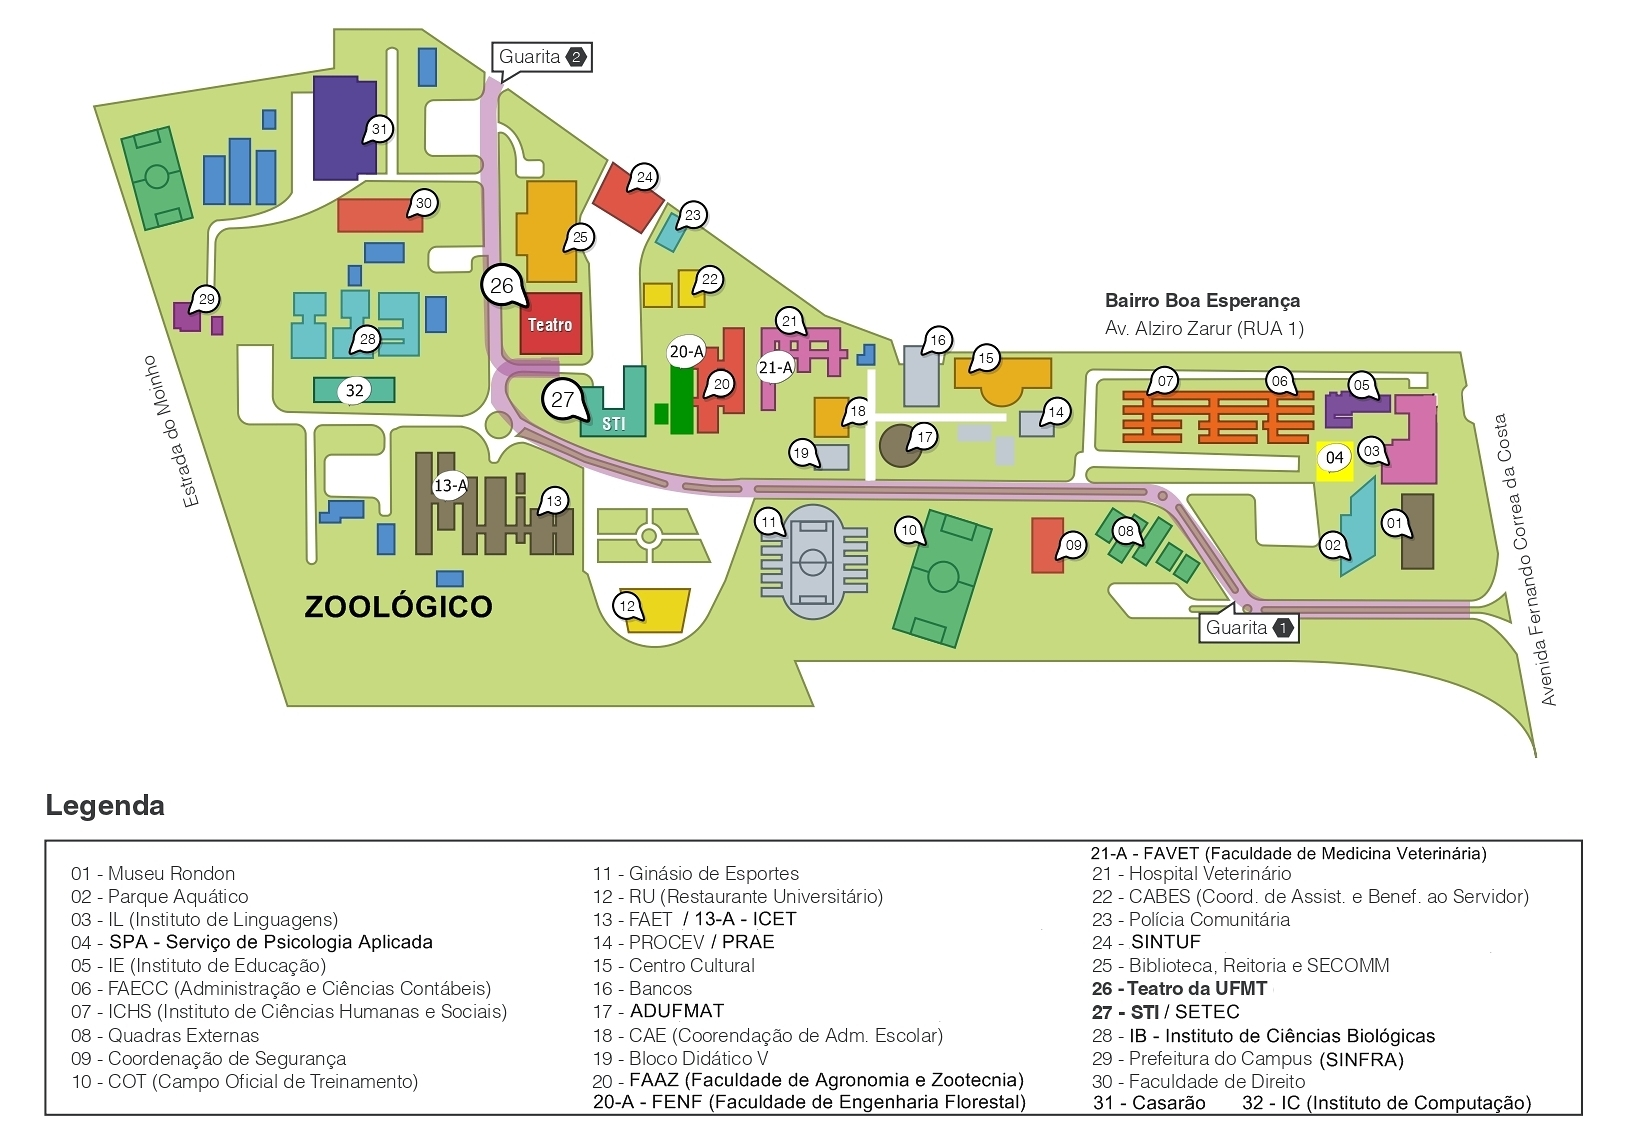
\includegraphics[scale=0.2]{figs/mapa.png}
\fonte{site da UFMT \url{https://ufmt.br/curso/comp/pagina/discente/8671}}
\end{figure}

Este parágrafo apresenta como referenciar a figura no texto, requisito
obrigatório da ABNT. 
Primeira opção, utilizando \texttt{autoref}: Ver o \autoref{figura_exemplo}. 
Segunda opção, utilizando  \texttt{ref}: Ver o Figura \ref{figura_exemplo}.

\section{Sobre o uso das chamadas de citações}
As citações e notas devem ser elaboradas conforme a ABNT NBR 10520. As citações diretas com até 3 linhas devem estar sempre dentro do texto identificadas entre “aspas”, somente se as citações ultrapassarem o limite de 3 linhas estas devem ser usadas com o recuo. Para as citações diretas com mais de 3 linhas que se enquadram para o uso do recuo, recomenda-se que este seja utilizado 4 cm da margem esquerda, apresentando tamanho menor de fonte e espaço simples entre linhas, sem aspas. Caso o autor venha a optar por outro tamanho de recuo o mesmo deve ser padronizado para todo o trabalho. Deve-se observar também que a chamada da citação deve vir antes (quando se usa por exemplo: de acordo com, conforme, entre outras opções com a sequência do nome do sobrenome do autor dentro do texto seguido de data e página (se houver) entre parênteses), ou depois da citação (quando se usa o sobrenome do autor seguido da data e página (se houver) entre parênteses, mas não devendo ser utilizada de forma repetida, ou seja, antes e depois para a mesma citação. A definição de como/onde a chamada de citação aparecerá no texto/parágrafo em que se apresenta uma citação direta, depende da forma como o autor está criando o texto.

\section{Uso do recurso Legendas para ilustrações e tabelas}
Para criar uma lista de ilustrações de forma automática, sugere-se a utilização do recurso de Legendas para colocar legendas nas ilustrações e tabelas. Desse modo será possível inserir o índice de ilustrações no início do trabalho e atualizar sempre que preciso. As ilustrações abaixo são apenas para exemplificar o uso do recurso.

Conforme estabelecido na ABNT NBR 14724:2011 sobre as ilustrações utilizadas no trabalho:
\begin{citacao}
Qualquer que seja o tipo de ilustração, sua identificação aparece na parte superior, precedida da palavra designativa (desenho, esquema, fluxograma, fotografia, gráfico, mapa, organograma, planta, quadro, retrato, figura, imagem, entre outros), seguida de seu número de ordem de ocorrência no texto, em algarismos arábicos, travessão e do respectivo título. Após a ilustração, na parte inferior, indicar a fonte consultada (elemento obrigatório, mesmo que seja produção do próprio autor), legenda, notas e outras informações necessárias à sua compreensão (se houver). A ilustração deve ser citada no texto e inserida o mais próximo possível do trecho a que se refere (Associação Brasileiras de Normas Técnicas, 2011, p. 11).
\end{citacao}

\chapter{CONSIDERAÇÕES FINAIS}\label{CONSIDERAÇÕES}
\textcolor{red}{Parte final do texto na qual se apresentam as conclusões apoiadas no desenvolvimento do assunto.
}

\chapter{SOBRE AS REFERÊNCIAS}\label{SOBRE}
\textcolor{red}{Elaborar referências de acordo com a NBR 6023:2018, esta parte do trabalho utiliza
alinhamento à esquerda, espaçamento entre linhas simples, ordenando as referências em
ordem alfabética e separando cada uma delas com um espaço de “Enter”. Caso o sistema de
chamada de citação utilizado ao longo do trabalho seja o Sistema Numérico, as referências
devem ser numeradas de acordo com a ordem sequencial em que aparecem no texto pela
primeira vez e colocadas em lista nesta mesma ordem.
Independente do tipo de material/documento referenciado, estes devem ficar na
sequência de ordem alfabética ou numérica, não devendo haver separação por tipo de
materiais. Nos exemplos abaixo a separação é apenas para demonstrar alguns dos vários tipos
de documentos que devem ser referenciados caso sejam utilizados/citados no decorrer do
trabalho.
Alguns exemplos de referências:}

\textcolor{red}{Livro:}
\begin{flushleft}
\begin{SingleSpace}
JÚNIOR, Rogério Henrique de. \textbf{Precisão no processo de busca e recuperação da informação}. Brasília: Thesaurus, 2007.
\end{SingleSpace}
\end{flushleft}

\begin{flushleft}
\begin{SingleSpace}
MARCONI, Marina de Andrade; LAKATOS, Eva Maria. \textbf{Metodologia científica:} ciência e conhecimento, métodos científicos, teoria, hipóteses e variáveis, metodologia jurídica. 6. ed. São Paulo: Atlas, 2011.
\end{SingleSpace}
\end{flushleft}

\textcolor{red}{Livro em meio eletrônico:}
\begin{flushleft}
\begin{SingleSpace}
OLIVEIRA, João Maria de; ARAUJO, Bruno Cesar de; SILVA, Leandro Valério. \textbf{Panorama da economia criativa no Brasil.} Rio de Janeiro: IPEA, 2013. Disponível em: \url{http://www.ipea.gov.br/portal/images/stories/PDFs/TDs/td_1880.pdf}. Acesso em: 10 jul. 2024.
\end{SingleSpace}
\end{flushleft}

\textcolor{red}{Capítulo de livro:}
\begin{flushleft}
\begin{SingleSpace}
CAMARGO, Liriane Soares de Araújo de; VIDOTTI, Silvana Aparecida Borsetti Gregório. Arquitetura da informação para repositórios científicos digitais. \textit{In}: SAYÃO, Luis (org.). \textbf{Implantação e gestão de repositórios institucionais:} políticas, memória, livre acesso e preservação. Salvador: EDUFBA, 2009. p. 55-82.
\end{SingleSpace}
\end{flushleft}

\textcolor{red}{Autoria de pessoa jurídica:}
\begin{flushleft}
\begin{SingleSpace} 
ASSOCIAÇÃO BRASILEIRA DE NORMAS TÉCNICAS. \textbf{NBR 14724:} informação e documentação: trabalhos acadêmicos: apresentação. Rio de Janeiro: ABNT, 2011.
\end{SingleSpace}
\end{flushleft}

\textcolor{red}{Dissertação:}
\begin{flushleft}
\begin{SingleSpace} 
FERNANDES, Joliza Chagas. \textbf{Representação da informação na WEB:} história da Paraíba nos sites Google e Alta Vista. 2004. Dissertação (Mestrado em Ciência da Informação) - Universidade Federal da Paraíba, João Pessoa, 2004.
\end{SingleSpace}
\end{flushleft}

\textcolor{red}{Parte de Evento:}
\begin{flushleft}
\begin{SingleSpace} 
KURAMOTO, Hélio. Acesso livre: maximizando a visibilidade das pesquisas e dos pesquisadores. \textit{In}: SEMINÁRIO EM CIÊNCIA DA INFORMAÇÃO, 3., 2009, Londrina. \textbf{Anais} [...]. Londrina: UEL, 2009. Disponível em: \url{http://www2.uel.br/eventos/secin/papers.php}. Acesso em: 15 jun. 2014.
\end{SingleSpace}
\end{flushleft}

\textcolor{red}{Artigo de periódico em meio eletrônico:}
\begin{flushleft}
\begin{SingleSpace} 
GRÁCIO, José Carlos Abbud; FADEL, Bárbara; VALENTIN, Marta Lígia Pomim. Preservação digital nas instituições de ensino superior: aspectos organizacionais, legais e técnicos. \textbf{Perspectivas em ciência da informação}, Belo Horizonte, v. 18, n. 3, p. 111-129, jul./set. 2013. Disponível em: \url{http://portaldeperiodicos.eci.ufmg.br/index.php/pci/article/
view/1612}. Acesso em: 13 set. 2019.
\end{SingleSpace}
\end{flushleft}

\textcolor{red}{Legislação em meio eletrônico}
\begin{flushleft}
\begin{SingleSpace} 
BRASIL. \textbf{Lei nº 14.133, de 01 de abril de 2021}. Lei de licitações e contratos. Brasília, DF: Presidência da República, 2021. Disponível em: \url{https://www.planalto.gov.br/ccivil_03/_ato2019-2022/2021/lei/l14133.htm}. Acesso em: 10 jul. 2024. 
\end{SingleSpace}
\end{flushleft}

\textcolor{red}{Mapa}
\begin{flushleft}
\begin{SingleSpace} 
ROHRBACH, Paulo Carlos (org.). \textbf{Mapa do estado de Mato Grosso}. Curitiba: Paranaense, 1970. 1 mapa, color., 137x47 cm. Escala 1:1.600.000.
\end{SingleSpace}
\end{flushleft}

\textcolor{red}{Essas referências foram adicionadas manualmente, mas caso queira usar um banco de dados de referências ".bib", abaixo será citado alguns tipos de referências contidas no arquivo "referencias.bib", e essas serão incorporadas de maneira automática na sessão de referências, na formatação adequada exigida pela ABNT. Se tiver preferência pela citação e referências numéricas, basta editar no preâmbulo do atual documento as preferências do pacote "abntex2cite", alterando "alf"  para "num".}

Livros: \cite{gomes1998,FUNDAP1994,koogan1998,brasileira1939,geografico1943,paulista1941,michalany1981}

Tese de doutorado: \cite{barcelos1998}

Uma seção intitulada de um livro. Como um conto dentro da coleção maior de contos que compõem o livro: \cite{romano1996}

Uma seção, como um capítulo, ou um intervalo de páginas dentro de um livro: \cite{santos1994,priberam1998,secretaria1999}

Artigo: \cite{costa1998,fraipont1998}

Um processo de conferência: \cite{redes1995}

Artigo publicado em anais de congressos: \cite{martin1997}

Patente: \cite{cruvinel1989}

Páginas da web, mas pode ser qualquer coisa, desde slides de palestras até anotações pessoais: \cite{kobayashi1998,espaciais1987}

Manuais: \cite{NBR10520:2002,abntex2classe,abntex2cite,abntex2cite-alf}

% ----------------------------------------------------------
% ELEMENTOS PÓS-TEXTUAIS
% ----------------------------------------------------------
% ----------------------------------------------------------
% Referências bibliográficas
% ----------------------------------------------------------
\bibliography{referencias}

% ----------------------------------------------------------
% Apêndices
% ----------------------------------------------------------

\begin{apendicesenv}

\chapter{Título 1}

\textcolor{red}{Elemento opcional. Deve ser precedido da palavra APÊNDICE, identificado por letras maiúsculas consecutivas, travessão e pelo respectivo título. Utilizam-se letras maiúsculas dobradas na identificação dos apêndices, quando esgotadas as letras do alfabeto.}

\chapter{Título 2}

\textcolor{red}{Elemento opcional. Deve ser precedido da palavra APÊNDICE, identificado por letras maiúsculas consecutivas, travessão e pelo respectivo título. Utilizam-se letras maiúsculas dobradas na identificação dos apêndices, quando esgotadas as letras do alfabeto.}

\end{apendicesenv}


% ----------------------------------------------------------
% Anexos
% ----------------------------------------------------------
\begin{anexosenv}

\chapter{Título 1}

\textcolor{red}{Elemento opcional. Deve ser precedido da palavra ANEXO, identificado por letras maiúsculas consecutivas, travessão e pelo respectivo título. Utilizam-se letras maiúsculas dobradas, na identificação dos anexos, quando esgotadas as letras do alfabeto.}

\chapter{Título 2}

\textcolor{red}{Elemento opcional. Deve ser precedido da palavra ANEXO, identificado por letras maiúsculas consecutivas, travessão e pelo respectivo título. Utilizam-se letras maiúsculas dobradas, na identificação dos anexos, quando esgotadas as letras do alfabeto.}

\end{anexosenv}


\end{document}
